El poder de \textbf{Rust} es que permite a los usuarios desarrollar rápidamente con estructuras seguras de memoria de alto nivel con bajo consumo de memoria y tiempos de ejecución rápidos. Sin embargo, también permite un control de grano fino si es necesario. Si un desarrollador realmente quiere, puede desactivar la seguridad de la memoria en Rust y continuar desarrollando y ejecutando programas Rust (aunque no se recomienda). Los \textbf{crates} de Rust no son una excepción a esto. El \textbf{framework Actix Web} nos expone a algunos conceptos subyacentes del servidor web, invitándonos a modificarlos de forma segura si es necesario. El lanzamiento de un servidor web básico con el marco web de \textbf{Actix} introducirá algunos conceptos nuevos que debemos abordar antes de comenzar a desarrollar nuestras funciones.

\section{Lanzamiento de un servidor web Actix básico}

Para admitir un servidor \textbf{web Actix}, necesitamos crear un nuevo proyecto Cargo. Para habilitar la ejecución de un servidor \textbf{Actix}, debemos definir las siguientes dependencias en el archivo \textbf{Cargo.toml}:


\begin{lstlisting}
[dependencies]
actix-web = "4.0.1"
actix-rt = "2.7.0"
\end{lstlisting}

\textbf{actix-web} es el marco principal que alberga las estructuras que definen las rutas y el servidor. \textbf{actix-rt} nos permite ejecutar todo en el subproceso actual.

El siguiente código es la implementación de ejemplo estándar que pone en marcha un servidor rápidamente mientras nos muestra las características del marco de forma concisa:

\begin{lstlisting}
use actix_web::{web, App, HttpRequest, HttpServer, Responder};
async fn saludo(req: HttpRequest) -> impl Responder {
	let nombre = req.match_info().get("nombre").unwrap_or("Mundo");
	format!("Hola {}!", nombre)
}

#[actix_rt::main]
async fn main() -> std::io::Result<()> {
	HttpServer::new(|| {
		App::new()
		.route("/", web::get().to(saludo))
		.route("/{nombre}", web::get().to(saludo))
	})
	.bind("127.0.0.1:8000")?
	.run()
	.await
}
\end{lstlisting}

Aquí, usamos las estructuras web de \textbf{Actix} para definir una vista que extrae datos de la solicitud. Luego, redefinimos nuestra función principal como una función asíncrona utilizando la macro de la caja \textbf{actix-rt}. Sin esta macro, el programa no se compilaría ya que las funciones principales no pueden ser asíncronas. Luego construimos un nuevo servidor y definimos las rutas asignándolas a la función que queremos. Luego nos vinculamos a una dirección, ejecutamos y luego esperamos el resultado.

Si bien la funcionalidad asíncrona es nueva, nos centraremos en esto más adelante en el capítulo. Por ahora, deberíamos centrar nuestra atención en el cierre que se pasa a la nueva función de la estructura \textbf{HttpServer}.

\section{Comprender los cierres}

Los cierres son esencialmente funciones; sin embargo, tienen algunas diferencias. Cabe señalar que las funciones se pueden definir sobre la marcha a través de || corchetes en lugar de () corchetes. Un ejemplo simple de esto es imprimir un parámetro:


\begin{lstlisting}
let test_function: fn(String) = |string_input: &str| {
	println!("{}", string_input);
};

test_function("test");
\end{lstlisting}

Lo que sucede aquí es que asignamos la variable \textbf{test\_function} a nuestra función que imprime la entrada. El tipo es un tipo \textbf{fn}. Hay algunas ventajas en esto. Debido a que es una variable que se asigna, podemos explotar los ámbitos.

Las funciones normales definidas por sí mismas están disponibles a través del archivo/módulo en el que se importan o definen. Sin embargo, habrá momentos en el desarrollo web en los que deseamos que la disponibilidad de la función se restrinja a una determinada duración. Cambiar el cierre a un alcance interno puede lograr esto fácilmente:

\begin{lstlisting}
{
	let test_function: fn(String) = |string_input: &str| {		
		println!("{}", string_input);
	};
}

test_function("test");
\end{lstlisting}


Aquí, la llamada de nuestra función está fuera del alcance, lo que dará como resultado una función que no se encuentra en este error de alcance.

Las definiciones de cierre tienen una sintaxis similar. Sin embargo, pueden ingresar parámetros e interactuar con variables externas en su alcance:

\begin{lstlisting}
let test = String::from("test");
let test_function = || {
	println!("{}", test);
};

test_function();
\end{lstlisting}

Tenga en cuenta que no hemos definido un tipo para la variable \textbf{test\_function}. Esto se debe a que un cierre es un tipo anónimo único que no se puede escribir. La analogía más cercana a un cierre es una estructura que alberga variables capturadas.

Los cierres también pueden tener valores de retorno con los que se puede interactuar como una función normal:

\begin{lstlisting}
let test = String::from("test");
let test_function = || {
	println!("{}", test);
	return test + &String::from(" case")
};

let outcome: String = test_function();
\end{lstlisting}

Aquí, el resultado denotará la cadena devuelta del cierre bajo la variable \textbf{test\_function}.

Ahora que tenemos una mayor comprensión de los cierres, podemos mirar hacia atrás a nuestra función principal con confianza. Sabemos que se está llamando a un cierre en la función \textbf{HttpServer::new}. Dado que la estructura de la aplicación es la línea final del cierre, la aplicación debe devolverse del cierre para que se activen las funciones de enlace y ejecución. Con esta información sobre los cierres, podemos estar un poco más seguros con la creación de nuestro servidor \textbf{HTTP}:


\begin{lstlisting}
#[actix_rt::main]
async fn main() -> std::io::Result<()> {
	HttpServer::new(|| {
		println!("function esta disparada");
		let app = App::new()
		.route("/", web::get().to(saludo))
		.route("/{name}", web::get().to(saludo));
		return app
	})
	.bind("127.0.0.1:8000")?
	.workers(3)
	.run()
	.await
}
\end{lstlisting}

Aquí, definimos la aplicación y la devolvemos, y arrojamos una declaración de impresión. Podemos hacer lo que queramos en el cierre siempre que devolvamos una estructura de aplicación construida. También agregamos una función de trabajadores con el parámetro 3. Cuando ejecutamos esto, podemos ver que obtenemos el siguiente resultado:

\begin{lstlisting}
    Finished dev [unoptimized + debuginfo] target(s) in 35.66s
Running `target/debug/web_rust`
function esta disparada
function esta disparada
function esta disparada
\end{lstlisting}


Esto nos dice que el cierre fue disparado tres veces. Alterar el número de trabajadores nos muestra que existe una relación directa entre este y el número de veces que se dispara el cierre. Si la función de los trabajadores se omite, el cierre se activa en relación con la cantidad de núcleos que tiene su sistema.

Ahora que comprendemos los matices en torno a la construcción de la estructura de la aplicación, es hora de ver el cambio principal en la estructura del programa, la programación asíncrona.

\section{Entender la programación asíncrona}

Hasta este capítulo, hemos estado escribiendo código de manera secuencial. Esto es lo suficientemente bueno para scripts estándar. Sin embargo, en el desarrollo web, la programación asíncrona es importante, ya que hay múltiples solicitudes a los servidores y las llamadas a la API introducen tiempo de inactividad. En algunos otros lenguajes, como Python, podemos construir servidores web sin tocar ningún concepto asíncrono. Si bien los conceptos asincrónicos se utilizan en estos marcos web, la implementación se define bajo el capó. Esto también es cierto para el marco de trabajo de Rust Rocket. Sin embargo, como hemos visto, se implementa directamente en Actix Web.

Cuando se trata de utilizar código asíncrono, hay dos conceptos principales que debemos entender:

\begin{itemize}
	\item \textbf{Procesos}: Un proceso es un programa que se está ejecutando. Tiene su propia pila de memoria, registros para variables y código.
	\item \textbf{Hilos(o subprocesos)}: un hilo o subproceso es un proceso ligero que un planificador gestiona de forma independiente. Sin embargo, comparte datos con otros hilos y el programa principal.
\end{itemize}



En esta sección, veremos los hilos para ver el efecto que tienen en nuestro código. Una de las mejores formas de explorar \textbf{subprocesos} en cualquier lenguaje de programación es codificar una breve pausa en cada \textbf{subproceso} y tiempo para procesar el programa en general. Podemos cronometrar nuestro programa Rust con el siguiente código:

\begin{lstlisting}
use std::{thread, time};

fn do_something(number: i8) -> i8 {
	println!("number {} is running", number);
	let two_seconds = time::Duration::new(2, 0);
	thread::sleep(two_seconds);
	return 2
}

fn main() {
	let now = time::Instant::now();
	let one: i8 = do_something(1);
	let two: i8 = do_something(2);
	let three: i8 = do_something(3);
	println!("time elapsed {:?}", now.elapsed());
	println!("result {}", one + two + three);
}
\end{lstlisting}

Aquí, definimos una función estándar que duerme. Debe tenerse en cuenta que aunque estamos llamando a la función de suspensión desde el módulo de subprocesos de la biblioteca estándar, no hay nada en este código que genere un subproceso todavía. En la función principal, iniciamos el temporizador, activamos tres funciones, luego detenemos el temporizador e imprimimos la suma de los resultados después. Con esto, obtenemos la siguiente salida:

\begin{lstlisting}
number 1 is running
number 2 is running
number 3 is running
time elapsed 6.000599893s
result 6
\end{lstlisting}

Esto no es sorprendente. Tenemos las funciones ejecutándose secuencialmente. Cada función duerme durante 2 segundos, y el tiempo total transcurrido al final de todo el proceso es de poco más de 6 segundos.

Ahora vamos a crear un hilo para cada función:


\begin{lstlisting}
use std::{thread, time};

use std::thread::JoinHandle;

fn do_something(number: i8) -> i8 {
	println!("number {} is running", number);
	let two_seconds = time::Duration::new(2, 0);
	thread::sleep(two_seconds);
	return 2
}

fn main() {
	let now = time::Instant::now();
	let thread_one: JoinHandle<i8> = thread::spawn(|| do_something(1));
	let thread_two: JoinHandle<i8> = thread::spawn(|| do_something(2));
	let thread_three: JoinHandle<i8> = thread::spawn(|| do_something(3));
	let result_one = thread_one.join();
	let result_two = thread_two.join();
	let result_three = thread_three.join();
	println!("time elapsed {:?}", now.elapsed());
	println!("result {}", result_one.unwrap() + result_two.unwrap() + result_three.unwrap());
}
\end{lstlisting}

Aquí puede ver que pasamos un cierre a través de cada hilo. Si intentamos y simplemente pasamos la función \textbf{do\_something} a través del hilo, obtenemos un error quejándose de que el compilador esperaba un cierre FnOnce<()> y encontró un i8 en su lugar. Esto se debe a que un cierre estándar implementa el rasgo público FnOnce<()>, mientras que nuestra función \textbf{do\_something} simplemente devuelve i8.

Cuando se implementa \textbf{FnOnce<()>}, el cierre solo se puede llamar una vez. Esto significa que cuando creamos un hilo, podemos asegurarnos de que el cierre solo se puede llamar una vez, y luego, cuando regresa, el hilo termina. Como nuestra función \textbf{do\_something} es la línea final del cierre, se devuelve i8. Sin embargo, debe tenerse en cuenta que el hecho de que se implemente el rasgo \textbf{FnOnce<()>} no significa que no podamos llamarlo varias veces. Este rasgo solo se llama si el contexto lo requiere. Esto significa que si tuviéramos que llamar al cierre fuera del contexto del hilo, podríamos llamarlo varias veces.

Una vez que hemos separado los tres subprocesos, obtenemos una estructura \textbf{JoinHandle} de las funciones de generación de cada subproceso que creamos. Llamamos a la función de unión para cada uno de ellos. La función de unión espera a que finalice el subproceso asociado. Luego imprimimos el tiempo transcurrido. Las funciones de combinación devuelven una estructura de resultado, por lo que deben desenvolverse para acceder al valor de retorno del cierre pasado al hilo. Luego sumamos estos resultados para imprimir el resultado final. Si no llamamos a la función de unión, el proceso principal se ejecutará y finalizará antes de que finalicen los subprocesos. Este código de subprocesamiento da el siguiente resultado:

\begin{lstlisting}
number 1 is running
number 2 is running
number 3 is running
time elapsed 2.000523086s
result 6
\end{lstlisting}

Como podemos ver, todo el proceso tardó poco más de 2 segundos en ejecutarse. Esto se debe a que los tres subprocesos se ejecutan simultáneamente. También podemos notar que el hilo tres se dispara antes que el hilo dos. No se preocupe si obtiene una secuencia de 1, 2, 3. Los hilos terminan en un orden indeterminado. La programación es determinista, sin embargo, hay miles de eventos que ocurren bajo el capó que requieren que la CPU haga algo. Como resultado, los intervalos de tiempo exactos que obtiene cada subproceso nunca son los mismos. Estos pequeños cambios se suman. Debido a esto, no podemos garantizar que los hilos terminen en un orden determinado.

La generación de subprocesos nos brinda una comprensión práctica de la programación asíncrona. Sin embargo, recordamos que el servidor web de Actix no utiliza esta sintaxis; define funciones con una sintaxis async y await. Para sentirnos más cómodos con el marco web, debemos analizar esta sintaxis.

\section{Entendiendo async y await}

La sintaxis async y await maneja los mismos conceptos cubiertos en la sección anterior, sin embargo, hay algunos matices. En lugar de simplemente generar hilos, creamos futuros y luego los manipulamos cuando sea necesario.

En informática, un futuro es un cálculo sin procesar. Aquí es donde el resultado aún no está disponible, pero cuando llamamos o esperamos, el futuro se completará con el resultado del cálculo. Los futuros también pueden denominarse promesas, retrasos o diferidos. Para explorar futuros, crearemos un nuevo proyecto Cargo y utilizaremos los futuros creados en el archivo \textbf{Cargo.toml}:

\begin{lstlisting}[language=bash]
[dependencies]
futures = "0.3.21"
\end{lstlisting}

Ahora que tenemos nuestro futuro, podemos definir nuestra propia función asíncrona en el archivo \textbf{main.rs}:

\begin{lstlisting}[language=bash]
async fn do_something(number: i8) -> i8 {
	println!("number {} is running", number);
	let two_seconds = time::Duration::new(2, 0);
	thread::sleep(two_seconds);
	return 2
}
\end{lstlisting}

Esta es la función de subproceso estándar que definimos anteriormente para señalar que el subproceso se está ejecutando y devuelve un valor del subproceso. La única diferencia es que tenemos una palabra clave asíncrona antes de la definición fn. La forma más sencilla de manejar esta función es llamarla y luego bloquear el programa hasta que finalice el cálculo:

\begin{lstlisting}[language=bash]
use futures::executor::block_on;
use std::{thread, time};

fn main() {
	let now = time::Instant::now();
	let future_one = do_something(1);
	let outcome = block_on(future_one);
	println!("time elapsed {:?}", now.elapsed());
	println!("Here is the outcome: {}", outcome);
}
\end{lstlisting}

Aquí, la variable \textbf{future\_one} es un futuro. Ejecutar esto nos da el siguiente resultado:

\begin{lstlisting}[language=bash]
number 1 is running
time elapsed 2.000196102s
Here is the outcome: 2
\end{lstlisting}

Esto es de esperar ya que es lo mismo que el resultado del subproceso en la sección anterior. El resultado de la función asíncrona también se puede extraer usando await. Para hacer esto, necesitamos tener un bloque asíncrono:

\begin{lstlisting}[language=bash]
// Agregar al programa main.rs
let future_two = async {
	return do_something(2).await
};    
let future_two = block_on(future_two);    
println!("Here is the outcome: {:?}", future_two);
\end{lstlisting}

Esto parece un poco detallado ya que está haciendo lo mismo que simplemente llamar a la función block\_on en el futuro desde la llamada a la función \textbf{do\_something}. Sin embargo, se puede llamar a \textbf{await} dentro de otra función asíncrona. También podemos ser más flexibles dentro del bloque asíncrono. Por ejemplo, podemos empaquetar dos futuros y devolverlos:

\begin{lstlisting}[language=bash]
let future_two = async {
	let outcome_two = do_something(2).await;  
	let outcome_three = do_something(3).await;
	return [outcome_two, outcome_three]    
};
let future_two = block_on(future_two);    
println!("Here is the outcome: {:?}", future_two);
\end{lstlisting}

Esto da la siguiente salida:

\begin{lstlisting}[language=bash]
number 2 is running
number 3 is running
Here is the outcome: [2, 2]
\end{lstlisting}

Sin embargo, si lo cronometramos, podemos ver que las funciones se activan de forma secuencial, lo que lleva poco más de 4 segundos. Esto no es muy útil, ya que es mejor que no nos molestemos con la sintaxis asíncrona si vamos a obtener los mismos resultados de tiempo que la programación secuencial normal.

Unirse parecía funcionar en la sección anterior. Dado que los futuros también tienen una función de combinación, tiene sentido utilizarla para dividir el tiempo necesario a la mitad haciendo que dos futuros se ejecuten al mismo tiempo:

\begin{lstlisting}[language=bash]
use futures::join;
...
let future_two = block_on(future_two);    
println!("Here is the outcome: {:?}", future_two);  
let second_outcome = async {
	let future_two = do_something(2);
	let future_three = do_something(3);
	return join!(future_two, future_three)
};    
let now = time::Instant::now();    
let result = block_on(second_outcome);    
println!("time elapsed {:?}", now.elapsed());    
println!("here is the result: {:?}", result);  
\end{lstlisting}

Sin embargo, esto no nos da el resultado que esperábamos:

\begin{lstlisting}[language=bash]
number 1 is running
time elapsed 2.000109916s
Here is the outcome: 2
number 2 is running
number 3 is running
Here is the outcome: [2, 2]
\end{lstlisting}

Los futuros se están ejecutando secuencialmente. La única diferencia es que devolvemos el resultado de los futuros en una tupla. A pesar de que la función \textbf{futures::join} es contraria a la intuición, podemos usar otra caja para crear nuestra propia función de unión asíncrona usando la caja \textbf{async\_std}. Antes de hacer esto, podemos definir la caja en la sección de dependencias del archivo \textbf{Cargo.toml}:

\begin{lstlisting}[language=bash]
async-std = "1.10.0"
\end{lstlisting}

Con esta caja, ahora podemos ejecutar nuestros futuros de forma asíncrona:

\begin{lstlisting}[language=bash]
use std::vec::Vec;
use async_std;
use futures::future::join_all;
...
        let mut futures_vec = Vec::new();
let future_four = do_something(4);
let future_five = do_something(5);
futures_vec.push(future_four);
futures_vec.push(future_five);
let handles = futures_vec.into_iter().map(async_std::task::spawn).collect::<Vec<_>>();
let results = join_all(handles).await;
return results    
};
let now = time::Instant::now();    
let result = block_on(third_outcome);    
println!("time elapsed for join vec {:?}", now.elapsed());    
println!("Here is the result: {:?}", result);
\end{lstlisting}

Aquí, lo que hemos hecho es definir nuestros futuros en un bloque asíncrono y luego agregarlos a un vector denominado \textbf{futures\_vec}. Luego obtenemos nuestro vector poblado de futuros y llamamos a la función \textbf{into\_iter} en él. Esto devuelve un iterador, que podemos usar para recorrer los futuros.

También podemos devolver un iterador simplemente llamando a la función iter. Sin embargo, llamar a esto producirá \textbf{\&T}. Simplemente hacer referencia a un futuro no es un futuro. Necesitamos el directorio futuro si vamos a aplicarle la función de generación. Nuestra función \textbf{into\_iter} nos permite obtener \textbf{T}, \textbf{\&T} o \textbf{\&mut T}, según el contexto y las necesidades.

Luego aplicamos la función \textbf{async\_std::task::spawn} a cada futuro en el vector usando la función de mapa. La función \textbf{async\_std::task::spawn} parece familiar para la función \textbf{thread::spawn} que usamos anteriormente, así que, nuevamente, ¿por qué molestarse con todo este dolor de cabeza adicional? Podríamos simplemente recorrer el vector y generar un hilo para cada tarea. La diferencia aquí es que la función \textbf{async\_std::task::spawn }genera una tarea asíncrona en el mismo hilo. Por lo tanto, ¡estamos ejecutando simultáneamente ambos futuros en el mismo hilo!

Luego usamos la función de recopilación para recopilar los resultados de este mapeo en un vector llamado identificadores. Una vez hecho esto, pasamos este vector a la función \textbf{join\_all} para unir todas las tareas asíncronas y esperar a que se completen usando \textbf{await}. Con esto, obtenemos la siguiente salida:

\begin{lstlisting}[language=bash]
number 1 is running
time elapsed 2.000157327s
Here is the outcome: 2
number 2 is running
number 3 is running
Here is the outcome: [2, 2]
number 2 is running
number 3 is running
time elapsed 4.000374497s
here is the result: (2, 2)
number 4 is running
number 5 is running
time elapsed for join vec 2.005101774s
Here is the result: [2, 2]
\end{lstlisting}

¡Hemos logrado ejecutar dos tareas asíncronas al mismo tiempo en el mismo hilo, lo que resultó en que ambos futuros se ejecutaran en poco más de 2 segundos!

Como podemos ver, generar hilos y tareas asíncronas en Rust es bastante sencillo. Sin embargo, debemos tener en cuenta que pasar variables a subprocesos y tareas asíncronas no es sencillo. El mecanismo de préstamo de Rust garantiza la seguridad de la memoria. Tenemos que pasar por pasos adicionales al pasar datos a un hilo. Una mayor discusión sobre los conceptos generales detrás del intercambio de datos entre subprocesos no es propicia para nuestro proyecto web. Sin embargo, podemos indicar brevemente qué tipos permiten esto:

\begin{lstlisting}[language=bash]
std::sync::Arc: Este tipo permite que los subprocesos hagan referencia a datos externos:

use std::sync::Arc;
use std::thread;

let names = Arc::new(vec!["dave", "chloe", "simon"]);
let reference_data = Arc::clone(&names);
let new_thread = thread::spawn(move || {
	println!("{}", reference_data[1]);
});

std::sync::Mutex: Este tipo permite a los subprocesos mutar datos externos:

use std::sync::Mutex;
use std::thread;

let count = Mutex::new(0);
let new_thread = thread::spawn(move || {
	*count.lock().unwrap() += 1;	
});
\end{lstlisting}

Dentro del hilo aquí, eliminamos la referencia del resultado del bloqueo, lo desenvolvemos y lo mutamos. Debe tenerse en cuenta que solo se puede acceder al estado compartido una vez que se mantiene el bloqueo.

Mirando hacia atrás en el servidor web básico que construimos en la sección anterior, hemos explorado casi todos los nuevos conceptos que se introdujeron. El último concepto que debe entenderse es la definición de la función principal. Podemos ver que la función principal es una función asíncrona. Sin embargo, si simplemente tratamos de definir la función principal como una función asíncrona, devolverá un futuro en lugar de ejecutar el programa.

Esto es posible gracias a la macro \textbf{\#[actix\_rt::main]} proporcionada por la caja \textbf{atix-rt}. Esta es una implementación de tiempo de ejecución y permite que todo se ejecute en el subproceso actual. La macro \textbf{\#[actix\_rt::main]} marca la función asíncrona (que en este caso es la función principal) para que la ejecute el sistema \textbf{Actix}.

A riesgo de meterse en problemas aquí, la caja Actix ejecuta un cálculo concurrente basado en el modelo actor. Aquí es donde un actor es un cómputo. Los actores pueden enviar y recibir mensajes entre ellos. Los actores pueden alterar su propio estado, pero solo pueden afectar a otros actores a través de mensajes, lo que elimina la necesidad de una sincronización basada en bloqueos (el mutex que cubrimos está basado en bloqueos). Una mayor exploración de este modelo no nos ayudará a desarrollar aplicaciones web. Sin embargo, la caja Actix tiene buena documentación sobre la codificación de sistemas concurrentes con Actix en \textbf{https://actix.rs/book/actix/sec-0-quick-start.html}.

Hemos cubierto mucho aquí. No te sientas estresado si no sientes que lo has retenido todo. Hemos cubierto brevemente una variedad de temas relacionados con la programación asíncrona. No necesitamos entenderlo de adentro hacia afuera para comenzar a construir aplicaciones basadas en el \textbf{framework Actix Web}.

Sin embargo, este recorrido rápido es invaluable cuando se trata de depurar y diseñar aplicaciones. Para ver un ejemplo en la naturaleza, podemos ver esta solución inteligente de desbordamiento de pila para ejecutar varios servidores en un solo archivo: \textbf{https://stackoverflow.com/questions/59642576/run-multiple-actix-app-on- different-ports}.

Las vistas básicas se definen para cada servidor. Como podemos ver, incluso si son dos servidores diferentes, no se necesita notación adicional:

\begin{lstlisting}[language=bash]
use actix_web::{web, App, HttpServer, Responder};
use futures::future;
async fn utils_one() -> impl Responder {
	"Utils one reached\n"	
}
async fn health() -> impl Responder {
	"All good\n"	
}
\end{lstlisting}

Una vez que se definen las vistas, los dos servidores se definen en la función principal:

\begin{lstlisting}[language=bash]
#[actix_rt::main]
async fn main() -> std::io::Result<()> {
	let s1 = HttpServer::new(move || {
		App::new().service(web::scope("/utils").route(
		"/one", web::get().to(utils_one)))	
	})
	.bind("0.0.0.0:3006")?
	.run();
	let s2 = HttpServer::new(move || {
		App::new().service(web::resource(
		"/health").route(web::get().to(health)))	
	})
	.bind("0.0.0.0:8080")?
	.run();
	future::try_join(s1, s2).await?;	
	Ok(())	
}
\end{lstlisting}

Podemos deducir con confianza que s1 y s2 son futuros que devuelve la función de ejecución. Luego unimos estos dos futuros y esperamos a que terminen. Con este ejemplo de la vida real, podemos ver que nuestra comprensión de la programación asíncrona nos permite desglosar lo que sucede cuando se construyen y ejecutan varios servidores.

Con nuestra nueva confianza en la programación asíncrona, no hay nada que nos impida crear 20 futuros y meterlos en un \textbf{try\_join}. macro para ejecutar 20 servidores, aunque esto no se recomienda, ya que aumentar la cantidad de servidores aumentará el uso de recursos con rendimientos decrecientes en el rendimiento.

Ahora que nos sentimos realmente cómodos con el marco \textbf{Actix Web}, prácticamente podemos considerar la creación de una aplicación escalable con él. Comenzaremos administrando las vistas de nuestra aplicación.

\section{Gestión de vistas mediante el marco Actix Web}

En la sección Lanzamiento de un servidor \textbf{web Actix básico}, definimos nuestras vistas en el archivo \textbf{main.rs}. Sin embargo, esto no es escalable. Si continuamos definiendo todas nuestras rutas en \textbf{main}, terminaremos con muchas importaciones y definiciones de ruta en un archivo. Esto hace que sea difícil de navegar y administrar. Si queremos cambiar un prefijo de \textbf{URL} para un bloque de vistas, la edición en este contexto es propensa a errores. Lo mismo ocurre con la desactivación de un bloque de vistas.

Para administrar nuestras vistas, necesitamos crear nuestros propios módulos para cada conjunto de vistas. Para administrar nuestras vistas, creamos un nuevo proyecto de Cargo llamado \textbf{administrando\_vistas}. Luego definimos la siguiente estructura del proyecto, ver figura \ref{cap2:001}.

\begin{figure}[htb]
	\centering
	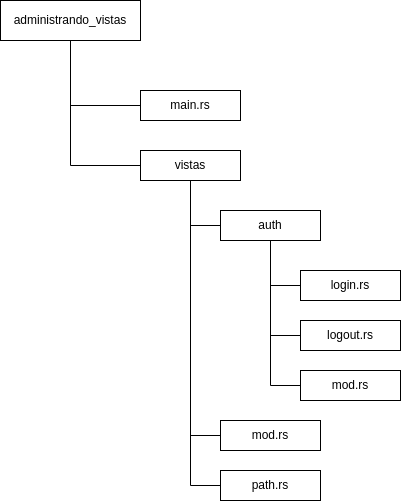
\includegraphics[width=0.4\textwidth]{capitulo2/estructura.png}
	\caption{Estructura básica de programa}
	\label{cap2:001}
\end{figure}

El archivo \textbf{main.rs} alberga nuestra definición del servidor. Luego definimos una estructura auxiliar de ruta de URL para todas nuestras vistas en el archivo \textbf{path.rs}. Definimos nuestras vistas de inicio y cierre de sesión en los archivos \textbf{login.rs} y \textbf{logout.rs}. Luego construimos las rutas a través de una función de fábrica en el archivo \textbf{vistas/auth/mod.rs}. Luego organizamos el disparo de la fábrica en una función de fábrica en el archivo \textbf{vistas/mod.rs}.

Ahora que nuestra estructura ha sido definida, podemos construir nuestro archivo \textbf{main.rs}:

\begin{lstlisting}[language=C]
use actix_web::{App, HttpServer};
mod vistas;
#[actix_rt::main]
async fn main() -> std::io::Result<()> {
	HttpServer::new(|| {
		let app = App::new();
		return app
	})
	.bind("127.0.0.1:8000")?
	.run()
	.await
}
\end{lstlisting}

Aquí, importamos nuestro módulo de vistas vacío, definimos nuestra aplicación en el cierre y la ejecutamos. Ejecutarlo ahora mismo nos dará un servidor sin vistas, por lo que podemos comenzar a trabajar en el módulo de vistas.

El primer archivo en el que podemos trabajar es el archivo vistas/path.rs, que alberga una estructura que define una ruta. Comenzamos aquí porque esta estructura no tiene dependencias. Esta estructura se utilizará para definir un prefijo estándar para una URL, que se fusiona con una cadena que se pasa a la función de definición para crear una cadena de URL:

\begin{lstlisting}[language=C]
pub struct Path {
	pub prefijo: String
}
impl Path {
	pub fn definir(&self, siguiendo_path: String) -> String {
		return self.prefijo.to_owned() + &siguiendo_path
	}
}
\end{lstlisting}

En nuestra función de definición, tomamos la referencia de la estructura como un parámetro \&self para que la misma instancia de estructura se pueda usar varias veces para definir varias URL con el mismo prefijo. Cabe señalar que las funciones con tales firmas se parecen a los métodos, lo que significa que se utilizan como métodos. También debe tenerse en cuenta que usamos una función \textbf{to\_owned} en la referencia al prefijo de la instancia de estructura. La función \textbf{to\_owned} crea datos propios a partir de datos prestados mediante la clonación. Queremos que nuestra función de definición devuelva una \textbf{URL} de cadena que se pueda pasar a otras funciones, sin embargo, también queremos que nuestra estructura \textbf{Path} conserve el atributo de prefijo para que pueda usarse nuevamente para otras vistas.

Ahora que hemos definido nuestra ruta, podemos pasar a nuestras vistas básicas de inicio y cierre de sesión. Nos acercamos a esto a continuación porque las vistas tampoco tienen dependencias. Teniendo en cuenta que este capítulo se centra en la gestión de vistas en lugar de iniciar y cerrar sesión, estas vistas simplemente devolverán una cadena. El procesamiento de datos en vistas se trata en el siguiente capítulo. La autenticación se trata en Gestión de sesiones de usuario.

En nuestro archivo \textbf{vistas/auth/login.rs}, definimos la siguiente vista de inicio de sesión:

\begin{lstlisting}[language=]
pub async fn login() -> String {
	format!("Vista Login")
}
\end{lstlisting}

Aquí, tenemos una función asíncrona estándar que devuelve una cadena. También podemos definir nuestra vista de cierre de sesión en el archivo \textbf{vistas/auth/logout.rs} de la misma manera:

\begin{lstlisting}[language=C]
pub async fn logout() -> String {
	format!("Vista Logout")
}
\end{lstlisting}

Ahora que hemos definido nuestras vistas, necesitamos crearlas en una función de fábrica en el archivo \textbf{vistas/auth/mod.rs}:

\begin{lstlisting}[language=C]
use actix_web::web;
mod login;
mod logout;
use super::path::Path;
pub fn fabrica_auth(app: &mut web::ServiceConfig) {
	let path_base: Path = Path{prefijo: String::from("/auth")};
	app.route(&path_base.definir(String::from("/entrar")), 
	web::get().to(login::login))
	.route(&path_base.definir(String::from("/salir")), 
	web::get().to(logout::logout));
}
\end{lstlisting}

En las importaciones, podemos notar que obtenemos la estructura \textbf{Path} del directorio principal del directorio \textbf{auth} usando \textbf{super}. Antes, hemos estado usando \textbf{super} para ingresar al archivo \textbf{mod.rs} en el mismo directorio. Sin embargo, si usamos \textbf{super} en un archivo \textbf{mod.rs}, entonces importamos archivos en el archivo \textbf{mod.rs }del directorio principal. Si quisiéramos, podríamos importar la estructura \textbf{Path} al archivo \textbf{vistas/auth/login.rs} usando \textbf{use super::super::path;}.

También podemos ver que una vez que hemos importado todo lo que necesitamos, definimos una función de fábrica que no devuelve nada y toma la aplicación para definir rutas en ella. Sin embargo, en lugar de pasar \textbf{actix\_web::App}, pasamos una estructura \textbf{actix\_web::web::ServiceConfig}. Incluso si intentamos pasar la estructura \textbf{actix\_web::App}, \textbf{actix\_web} no nos lo permitirá.

Una de las estructuras necesarias para definir el tipo de la función para pasar la aplicación es privada. La estructura \textbf{actix\_web::web::ServiceConfig} nos permite configurar más la aplicación. Usamos esto para definir rutas, sin embargo, podemos establecer datos de aplicaciones, registrar un servicio HTTP o registrar un recurso externo para recursos de generación de URL usando esta estructura.

Una vez que hemos pasado la estructura de configuración, definimos las rutas como lo haríamos si estuviéramos definiendo una ruta en el archivo \textbf{main.rs} donde está la definición del servidor. También podemos ver cómo se usa la estructura \textbf{Path}. Hay una ligera ventaja en el uso de la estructura \textbf{Path}. El prefijo de \textbf{URL} se define una vez, lo que reduce la posibilidad de que ocurra algún error tipográfico en el prefijo si estamos definiendo muchas rutas. También facilita el mantenimiento. Si vamos a cambiar un prefijo para un conjunto de vistas, solo tenemos que cambiarlo una vez en la construcción de la estructura \textbf{Path} en la fábrica.

Ahora que tenemos nuestro módulo de \textbf{vistas/autenticación} completamente operativo, simplemente podemos pasar la estructura de configuración a través de la fábrica para construir todas las rutas para la autenticación. En el futuro, también construiremos otros módulos para vistas. Debido a esto, necesitamos otra fábrica que pueda orquestar las fábricas de vistas múltiples. Esto se puede definir en el archivo \textbf{vistas/mod.rs}:

\begin{lstlisting}[language=C]
use actix_web::web;
mod path;
mod auth;
pub fn fabrica_vistas(app: &mut web::ServiceConfig) {
	auth::fabrica_auth(app);
}
\end{lstlisting}

Como podemos ver, importamos el módulo de autenticación y lo usamos para construir nuestras vistas en la fábrica. Observamos que pasamos la estructura de configuración a la fábrica y luego la pasamos a \textbf{fabrica\_auth}. El parámetro de la aplicación se puede pasar a varias fábricas una tras otra, ya que es una referencia y las fábricas se llaman en orden secuencial. También importamos el archivo de ruta. Si bien esto no se usa en el archivo, lo necesitamos para la súper llamada en la fábrica de autenticación. Es por eso que no recibimos una advertencia cuando ejecutamos el código.

Ahora tenemos una forma escalable y bien estructurada de administrar nuestras vistas, todo lo que tenemos que hacer es importar esta fábrica de vistas y llamarla en el archivo \textbf{main.rs}:

\begin{lstlisting}[language=C]
use actix_web::{App, HttpServer};
mod vistas;
#[actix_rt::main]
async fn main() -> std::io::Result<()> {
	HttpServer::new(|| {
		let app = App::new().configure(vistas::vistas fabrica)
		return app
	})
	.bind("127.0.0.1:8000")?
	.run()
	.await
}
\end{lstlisting}

Como podemos ver, esto es más o menos lo mismo. Todo lo que tenemos que hacer es llamar a la función de configuración en la estructura de la aplicación. Luego pasamos la fábrica de vistas a la función de configuración, que pasará la estructura de configuración a nuestra función de fábrica por nosotros. Como la función de configuración devuelve Self, es decir, la estructura de la aplicación, podemos devolver el resultado al final del cierre.

¡Ahora tenemos un servidor en funcionamiento que crea vistas de forma escalable! Simplemente podemos cortar todas nuestras vistas de autenticación simplemente comentando la siguiente línea en el archivo \textbf{vistas/mod.rs}:
\begin{lstlisting}[language=C]
auth::fabrica_auth(app);
\end{lstlisting}


Esto también nos da mucha flexibilidad. Al definir nuestras propias fábricas para cada módulo de vistas, no hay nada que nos impida agregar parámetros adicionales a las fábricas individuales para personalizar la compilación. Por ejemplo, si por alguna razón queremos deshabilitar la función de cierre de sesión en función de una variable de entorno o configuración, simplemente podemos agregar un condicional en nuestra fábrica en el archivo \textbf{vistas/auth/mod.rs}:

\begin{lstlisting}[language=C]
use actix_web::web;
mod login;
mod logout;
use super::path::Path;
pub fn fabrica_auth(app: &mut web::ServiceConfig, logout: bool) {
	let path_base: Path = Path{prefijo: String::from("/auth")};
	let app = app.route(&path_base.definir(String::from("/entrar")), 
	web::get().to(login::login))
	if logout {
		app.route(&path_base.definir(String::from("/salir")), 
		web::get().to(logout::logout));
	}
}
\end{lstlisting}

Todo lo que tenemos que agregar es un parámetro de cierre de sesión. Luego asignamos el resultado de la función de ruta a la variable de la aplicación. Luego llamamos a la función de ruta en esa variable si la variable de cierre de sesión es verdadera. Recuerda, no tenemos que devolver nada; solo necesitamos llamar a las funciones.

Es importante mantener la lógica aislada. La lógica para construir las vistas para el módulo de autenticación permanece en la fábrica de autenticación. Sin embargo, la colección de variables alrededor de la configuración debe definirse en \textbf{vistas/mod.rs}:

\begin{lstlisting}[language=C]
use actix_web::web;
mod path;
mod auth;
use std::env;
pub fn fabrica_vistas(app: &mut web::ServiceConfig) {
	let args: Vec<String> = env::args().collect();
	let param: &String = &args[args.len()-1];
	if param.as_str() == "cancel_logout" {
		println!("Vista logout no fue configurado");
	} else {
		println!("vista logout esta siendo configurada");
		auth::fabrica_auth(app, true);
	}
}
\end{lstlisting}

Aquí, recopilamos los parámetros del entorno. Si es \textbf{cancel\_logout}, la vista de cierre de sesión no se configurará. Mantener la lógica de los parámetros en la fábrica de \textbf{vistas/mod.rs} aumenta la flexibilidad al permitirnos configurar varias fábricas con un solo parámetro. También podemos revisar la estructura \textbf{Path} y la ventaja que ofrece aquí. Si tuviéramos que cambiar el prefijo de un conjunto de vistas sobre la marcha, solo necesitaríamos una declaración condicional o de coincidencia para la estructura Path al comienzo de la función de fábrica en lugar de cada función de definición de ruta.

Nuestro objetivo era crear una aplicación básica que sirva y gestione las vistas de forma escalable. Aquí, tenemos una aplicación que sirve vistas. Estas vistas pueden entrar y salir y definirse en sus propios módulos. Para ejecutar sin la vista de cierre de sesión, usamos la siguiente línea de comando:

\begin{lstlisting}[language=C]
cargo run cancel_logout
\end{lstlisting}

Si no, entonces solo ejecutamos la ejecución de carga. Si ejecutamos nuestra aplicación con la vista de cierre de sesión configurada, tenemos las siguientes URL y salidas:


\begin{lstlisting}[language=C]
http://127.0.0.1:8000/auth/login
\end{lstlisting}

Esto da la siguiente cadena:

\begin{lstlisting}[language=C]
Login view
\end{lstlisting}

También da esto:

\begin{lstlisting}[language=C]
http:/ /127.0.0.1:8000/auth/salir
\end{lstlisting}

Nosotros obtenemos la siguiente cadena:

\begin{lstlisting}[language=C]
Logout view
\end{lstlisting}

\section{Poniendo todo junto}

Hemos cubierto mucho para obtener algunas vistas básicas en funcionamiento en un servidor web Actix. Podríamos haber hecho todo esto en una página:

\begin{lstlisting}[language=C]
use actix_web::{web, App, HttpRequest, HttpServer, Responder};
pub async fn logout() -> String {
	format!("Vista de Salida")
}
pub async fn login() -> String {
	format!("Vista de entrada")
}
#[actix_rt::main]
async fn main() -> std::io::Result<()> {
	HttpServer::new(|| {
		let app = App::new()
		.route("/auth/entrar", web::get().to(login))
		.route("/auth/salir", web::get().to(logout));
		return app
	})
	.bind("127.0.0.1:8000")?
	.run()
	.await
}
\end{lstlisting}
